\section{Имитовставка (MAC)}\label{section-MAC}
\selectlanguage{russian}
\index{имитовставка}

Для обеспечения целостности и подтверждения авторства информации, передаваемой по каналу связи, используют \emph{имитовставку} $\MAC$ (\langen{Message Authentication Code}).

Имитовставкой называется \emph{криптографическая хэш-функция} $\MAC(K,m)$, зависящая от передаваемого сообщения $m$ и секретного ключа $K$ отправителя $A$, обладающая свойствами цифровой подписи:
\begin{itemize}
    \item получатель $B$, используя такой же или другой ключ, имеет возможность проверить целостность\index{целостность} и доказать принадлежность информации $A$;
    \item имитовставку невозможно фальсифицировать.
\end{itemize}

Имитовставка может быть построена либо на симметричной криптосистеме (в таком случае обе стороны имеют один общий секретный ключ), либо на криптосистеме с открытым ключом, в которой $A$ использует свой секретный ключ, а $B$ -- открытый ключ отправителя $A$.

Наиболее универсальный способ аутентификации сообщений через схемы ЭП на криптосистемах с открытым ключом состоит в том, что сторона $A$ отправляет стороне $B$ сообщение
    \[ m ~\|~ \textrm{ЭП}(K, h(m)), \]
где $h(m)$ -- криптографическая хэш-функция в схеме ЭП и $\|$ является операцией конкатенации битовых строк. Для аутентификации большого объёма информации этот способ не подходит из-за медленной операции вычисления подписи. Например, вычисление одной ЭП на криптосистемах с открытым ключом занимает порядка 10 мс на ПК. При средней длине IP-пакета 1 Кбайт, для каждого из которых требуется вычислить имитовставку, получим максимальную пропускную способность в $\frac{1 ~ \text{Кбайт}}{10 ~ \text{мс}} = 100$ Кбайт/с.

Поэтому для большого объёма данных, которые нужно аутентифицировать, $A$ и $B$ создают общий секретный ключ аутентификации $K$. Далее имитовставка вычисляется либо с помощью модификации блочного шифра, либо с помощью криптографической хэш-функции.

Для каждого пакета информации $m$ отправитель $A$ вычисляет $\MAC(K,m)$ и присоединяет его к сообщению $m$:
    \[ m ~ \|~ \MAC(K,m). \]
Зная секретный ключ $K$, получатель $B$ может удостовериться с помощью кода аутентификации, что информация не была изменена или фальсифицирована, а была создана отправителем.

Требования к длине кода аутентификации в общем случае такие же, как и для криптографической хэш-функции, то есть длина должна быть не менее 160--256 бит. На практике часто используют усечённые имитовставки.

Стандартные способы использования имитовставки сообщения следующие.
\begin{itemize}
    \item Если шифрование данных не применяется, отправитель $A$ для каждого пакета информации $m$ отсылает сообщение
        \[ m ~\|~ \MAC(K, m) .\]
    \item Если используется шифрование данных симметричной криптосистемой с помощью ключа $K_e$, то имитовставка с ключом $K_a$ может вычисляться как до, так и после шифрования:
        \[ E_{K_e}(m) ~\|~ \MAC(K_a, E_{K_e}(m)) ~~ \text{ или } ~~ E_{K_e}(m ~\|~ \MAC(K_a, m)). \]

\end{itemize}
Первый способ, используемый в IPsec\index{протокол!IPsec}, хорош тем, что для проверки целостности достаточно вычислить только имитовставку, тогда как во втором случае перед проверкой необходимо дополнительно расшифровать данные. С другой стороны, во втором способе, используемом в системе PGP\index{протокол!PGP}, защищённость имитовставки не зависит от потенциальной уязвимости алгоритма шифрования.

Вычисление имитовставки от пакета информации $m$ с использованием блочного шифра $E$ осуществляется в виде:
    \[ \MAC(K, m) = E_K(H(m)), \]
где $H$ -- криптографическая хэш-функция.

Имитовставка на основе хэш-функции обозначается $\HMAC$ (Hash-based MAC)\index{HMAC} и стандартно вычисляется в виде:
    \[ \HMAC(K, m) = H(K \| H(K \| m)). \]

Возможно также вычисление в виде:
    \[ \HMAC(K, m) = H(K \| m \| K). \]

В протоколе IPsec\index{протокол!IPsec} используется следующий способ вычисления кода аутентификации:
    \[ \HMAC(K, m) = H((K \oplus ~ \textrm{opad}) ~\|~ H((K \oplus ~ \textrm{ipad}) ~\|~ m)), \]
где $\textrm{opad}$ -- последовательность повторяющихся байтов
    \[ \text{\texttt{0x5C}}= [01011100]_2, \]
$\textrm{ipad}$ -- последовательность повторяющихся байтов
    \[ \text{\texttt{0x36}} = [00110110]_2, \]
которые инвертируют половину битов ключа. Считается, что использование различных значений ключа повышает криптостойкость.

В протоколе защищённой связи SSL/TLS\index{протокол!SSL/TLS}, используемом в интернете для инкапсуляции протокола HTTP\index{протокол!HTTP} в протокол SSL (HTTPS\index{протокол!HTTPS}), код $\HMAC$ определяется почти так же, как в IPsec. Отличие состоит в том, что вместо операции XOR для последовательностей $\textrm{ipad}$ и $\textrm{opad}$ осуществляется конкатенация:
    \[ \HMAC(K, m) = H((K ~\|~ \textrm{opad}) ~\|~ H((K ~\|~ \textrm{ipad}) ~\|~ m)). \]

Двойное хэширование\index{двойное хэширование} с ключом в
    \[ \HMAC(K, m) = H(K \| H(K \| m)) \]
применяется для защиты от атаки на расширение сообщений. Вычисление хэш-функции от сообщения $m$, состоящего из $n$ блоков $m_{1}, m_2 \dots m_n$, можно записать в виде:
\[\begin{array}{l}
	m \equiv m_1 \Vert m_2 \Vert \dots \Vert m_n, \\
	H_0 \equiv IV = \textrm{const}, \\
	H_i = f(H_{i-1}, m_i), i \in \{ 1, 2, \dots, n \},\\
	H(m) \equiv H_n,
\end{array}\]
где $f$ -- известная сжимающая функция.

Пусть имитовставка использует одинарное хэширование с ключом:
    \[ \MAC(K, m) = H(K \| m) = H (m_0 = K \| m_1 \| m_2 \| \dots \| m_n). \]
Тогда криптоаналитик, не зная секретного ключа, имеет возможность вычислить имитовставку для некоторого расширенного сообщения $m \| m_{n+1}$:
\[
    \MAC(K, m \| m_{n+1}) = \underbrace{H \left( K \| m_1 \| m_2 \| \dots \| m_n \right.}_{\MAC(K, m)} \left. \| m_{n+1} \right) =
\] \[
     = f(\MAC(K, m), m_{n+1}).
\]

\subsection{Универсальные хэш-функции}\label{sec:universal-hash-functions}
\selectlanguage{russian}
Наличие одного единственного правила хэширования может привести к тому, что злоумышленник, зная точную формулу вычисления хэша, сможет подобрать такой набор входных данных, который с большой степенью вероятности даёт коллизии обычной (не криптографической) хэш-функции. Кроме того, сами хэш-функции также разрабатываются исходя из определённого предположения о входных данных. Алгоритмы хэширования могут содержать некоторые константы, которые разработчику информационной системы предлагается выбрать самостоятельно, основываясь на его предположениях об особенностях входных данных. Но квалификации разработчика, либо его априорных знаний, может не хватать для эффективного выбора конкретной реализации (алгоритм и параметры) хэширования. Исходя из этого Картер и Вегман в 1979 году (\langen{John Lawrence Carter, Mark N. Wegman}, \cite{Carter:Wegman:1979}) предложили определить класс алгоритмов хэширования с возможностью выбора одного из них непосредственно в момент вызова.

Обозначим через $\delta$ возможный факт совпадения значения некоторой унарной функции для некоторых значений аргументов:

\[
\delta_{f}( x, y ) = \left\{\begin{matrix}
1, & f(x) = f(y);\\ 
0, & f(x) \neq f(y).
\end{matrix}\right.
\]

Пусть $H$ -- класс функций, преобразующих $M \to R$. Будем называть класс $H$ универсальным$_{2}$, если

\[
\forall x, y \in M: \sum_{h \in H} \delta_{h}( x, y ) \leq |H| / |R|.
\]

То есть класс функций $H$ универсален$_{2}$, если для любых пар аргументов $x$ и $y$ значения функций совпадают не более чем для $1/|R|$-ой части функций из множества $H$. Нижний индекс <<$_{2}$>> подчёркивает тот факт, что речь идёт о совпадении значений только для пар элементов. В дальнейшем мы его будем опускать.

Примеры универсальных классов для хэширования:\footnote{Универсальность первых двух примеров была показана ещё в работе Картера и Вегмана~\cite{Carter:Wegman:1979}. Последний описан, например, в~\cite{Dietzfelbinger:Gil:Matias:Pippenger:1992}.}

\begin{itemize}
    \item функции хэширования для чисел $x$
    \[ \begin{array}{l}
    h(x) = ax + b \bmod p,\\
    a \in \Z^*_p, b \in \Z_p;\\
    \end{array} \]
    \item функции хэширования для векторов $\vec{x}$
    \[ \begin{array}{l}
    \vec{x} = \left \langle x_0, x_1, \dots, x_r \right \rangle,\\
    \vec{a} = \left \langle a_0, a_1, \dots, a_r \right \rangle,\\
    \forall i \in \Z_{r+1}: a_i \in \Z_{p},\\
    h( \vec{x} ) = \sum_{i=0}^{r} a_i x_i \bmod p;\\
    \end{array} \]
    \item функции хэширования для строк (последовательностей переменной длины) $\vec{x}$
    \[ \begin{array}{l}
    \vec{x} = \left \langle x_0, x_1, \dots, x_l \right \rangle,\\
    \forall x_i: x_i \in \Z_{u}, \\
    p \geq u, \\
    a \in \Z_{p}, a \neq 0,\\
    h( \vec{x} ) = \sum_{i=0}^{l} a^{i} x_i \bmod p.\\
    \end{array} \]
\end{itemize}

На основе универсального хэширования построены такие криптографические примитивы, как UMAC и Poly1305 (RFC 8439).


\subsection{Одноразовая имитовставка}\label{sec:one-time-mac}
\selectlanguage{russian}
Одноразовый MAC (\langen{One-Time MAC}) можно рассматривать как аналог одноразового шифрблокнота для целей аутентификации сообщения. Если использовать один ключ для ровно одного сообщения, можно построить код аутентификации, который гарантированно не может быть подделан злоумышленником.

Если сообщение короткое, то можно считать ключом два числа $a$ и $b$, а в качестве значения MAC для сообщения $m \in M$ будет выступать
\[
h(m) = a \times m + b \bmod p.
\]

Если $p$ -- простое, то вероятность угадать значение MAC для некоторого сообщения $m_2$ (то есть подменить сообщение $m_1$ с одновременной генерацией нового MAC) без знания ключа $k=\overrightarrow{(a,b)}$, равна строго $1/p$.

Можно воспользоваться описанной ранее функцией хэширования для сообщений переменной длины и использовать чуть более сложную формулу для вычисления MAC:

\[ \begin{array}{l}
\vec{m} = \left \langle m_1, m_2, \dots, m_l \right \rangle, \\
h(\vec{m}) = b + \sum_{i=1}^{l} a^i m_i \mod p. \\
\end{array}  \]

Для этой формулы по прежнему сохраняется свойство, что если ключ $k=\overrightarrow{(a,b)}$ используется ровно один раз, злоумышленник не сможет подделать (угадать) MAC с вероятностью более $1/p$.


\subsection{Конструкция Вегмана-Картера}
\selectlanguage{russian}

В 1981 году Вегман и Картер предложили (\cite{Wegman:Carter:1981}) использовать универсальное хэширование (раздел~\ref{sec:universal-hashing}) для построение алгоритмов имитовставок. В оригинале авторы предполагали, что каждое сообщение содержит неповторяющийся номер $i$, а секретный ключ между отправителем и получателем состоит из двух частей:

\begin{itemize}
    \item параметра $k_1$, задающего способ выбора функции из универсального класса хэширования $H: K \times A \to B$;
    \item параметра $k_2$, который является \emph{последовательностью} строк $b_1, b_2, \dots, b_n$, длина каждой из которых совпадает с размером элементов множества $B$.
\end{itemize}

Результатом вычисления имитовставки является:

\[ \begin{array}{l}
    m' = \langle i, m \rangle,\\
    \textrm{MAC} (m') = H_{k_1}(m) \oplus b_i.
\end{array} \]

Авторы показали надёжность данной схемы при условии случайного выбора ключей и универсальности класса хэширования. Однако с практической точки зрения использовать ключи, состоящие из \emph{последовательностей} очень непрактично. Более того, можно было передать столько сообщений, сколько элементов последовательности задано в $k_2$. Для передачи сообщения сверх этого лимита нужно было либо расширить существующий ключ, либо сгенерировать новый.

По этой причине сейчас вместо использования последовательности строк $b_1, b_2, \dots, b_n$ в качестве ключа предполагается наличие некоторого класса псевдослучайных функций (\langen{pseudorandom function family, PRF}), который эмулирует \emph{случайного оракула}\index{оракул!случайный}. В своей идеализированной модели он для каждого некоторого входа может выдать ответ, случайно распределённой по области значений. Однако если на вход случайного оракула будет подано уже ранее подававшееся значение, он должен выдать прежний ответ. Входом этого оракула являются, во-первых, некоторое случайное число $r$, которое заменило собой номер сообщения, во-вторых часть общего секретного ключа $k_2$, которая будет служить для выбора конкретной функции из класса псевдослучайных.

В качестве практической реализации такого класса функций могут, с некоторым приближением, выступать другие реализации имитовставок, даже если они медленно работают. Например, основанные на криптографических хэш-функциях или блочных шифрах. Потому что им на вход (в отличие от быстрой функции универсального хэширования) подаётся только небольшой блок информации -- случайное число $r$.

Таким образом, современную конструкцию Вегмана-Картера можно описать так. Пусть выбран некоторый класс универсальных хэш-функций (например, в качестве него можно использовать одноразовую имитовставку из раздела~\ref{sec:one-time-mac}) \[
    H: \{0,1\}^{|k_1|} \times \{0,1\}^* \to \{0,1\}^n,
\] и некоторая надёжная реализация медленной имитовставки \[
    PRF: \{0,1\}^{|k_2|} \times \{0,1\}^{|r|} \to \{0,1\}^n.
\]

Тогда получение быстрой имитовставки можно сделать следующим образом
\[ \begin{array}{l}
\textrm{secret key: } k: \langle k_1, k_2 \rangle,\\
\textrm{random nonce: } r \leftarrow {0,1}^n,\\
\textrm{MAC} (m) = \langle r, H_{k_1}(m) \oplus PRF_{k_2}(r) \rangle.
\end{array} \]

Как утверждается в~\cite{Krovetz:2000}, использование данной конструкции позволяет достичь скорости хэширования в $0{,}5$ циклов процессора на один байт сообщения (\langen{cycles per byte, cpb}).


\subsection{UMAC}\label{sec:umac}
\selectlanguage{russian}

Конструкция UMAC, предложенная в 1999 году (\cite{Black:Halevi:Krawczyk:etc:1999}), также использует подход с быстрым универсальным хэшированием большого исходного сообщения и хэшированием небольшого блока информации надёжной (на 1999 год), но медленной ключевой функцией HMAC-SHA1. В 2003 году вошёл в список алгоритмов, отобранных инициативой NESSIE (\langen{New European Schemes for Signatures, Integrity, and Encryptions}) как безопасный алгоритм вычисления имитовставки. В 2006 году был стандартизован как RFC~4418 (\cite{rfc4418}). На сегодняшний день не считается криптографически стойким из-за уязвимостей, найденных в SHA-1.

Используемый в UMAC универсальный$_2$ класс хэш-функций $\textrm{NH}_K (m)$ описывается следующим образом. Битовая строка $m$ длиной до 1024 32-битовых <<слов>> и размером, кратная 2 <<словам>>, разбивается на отдельные блоки по 32 бита $m_1, m_2, \dots, m_l$. 32-битные ключи $K_1, K_2, \dots, K_l$ получаются из исходного ключа $K$ с помощью генератора псевдослучайных чисел. Далее вычисление 64-битового хэша выглядит так: \[\begin{array}{ll}
    \textrm{NH}_K (m) = & ( m_1 +_{32}K_1) \times_{64} (m_2 +_{32} K_2) +_{64} \dots \\
                        & \dots ~ +_{64} ~ \dots \\
                        & \dots ~ +_{64} ~ (m_{l-1} +_{32} K_{l-1}) \times_{64} (m_l+_{32}K_l),
\end{array} \] где $+_{32}$ -- сложение 32-битных строк, в результате которого получается 32-битная сумма, $\times_{64}$ -- произведение двух 32-битных строк, и получаемый 64-битный результат умножения (рис.~\ref{fig:UMAC}).

\begin{figure}
    \centering
    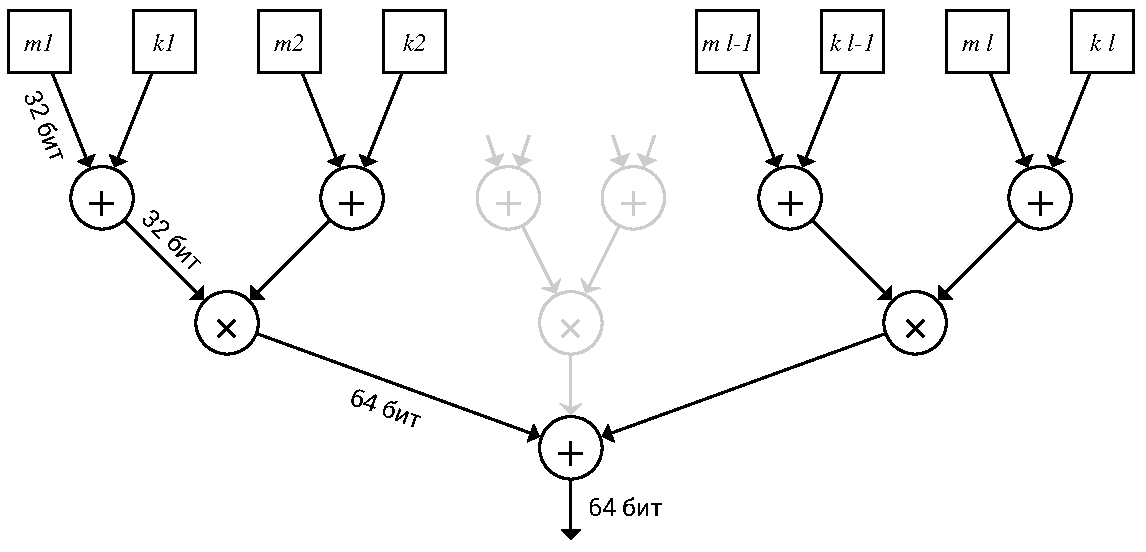
\includegraphics[width=1\textwidth]{pic/UMAC}
    \caption{Универсальное хэширование $\textrm{NH}_K (m)$ в UMAC}
    \label{fig:UMAC}
\end{figure}

Генерация имитовставки делается следующим образом. Предполагается, что вместе с сообщением $m$ передаётся случайная строка \emph{nonce} (должна быть уникальна для каждого сообщения), а у отправителя и получателя есть общий секретный ключ $K$.

\begin{enumerate}
    \item Пусть Len это остаток от деления длины сообщения в битах $|m|$ на 4096:\[
        \textrm{Len} = |m| \bmod 4096.
    \]
    \item Сообщение $m$ в битовом представлении дополняется нулями таким образом, чтобы длина сообщения $|m|$ была кратна 64 бит (8 байт).
    \item Сообщение $m$ разбивается на блоки по 32768 бита (1024 <<слова>> по 32 бита) $m_1, m_2, \dots, m_t$. Последний блок будет содержать от 2 до 1024 <<слов>>.
    \item Каждый блок хэшируется ключевой хэш-функцией $\textrm{NH}_K$, результаты конкатенируются между собой и $Len$:\[
        H_K(m) = \textrm{NH}_K (m_1) ~ \| ~ \textrm{NH}_K (m_2) ~ \| ~ \dots ~ \| ~ \textrm{NH}_K (m_t) ~ \| ~ \textrm{Len}.
    \]
    \item Итоговое значение имитовставки получается через хэширование ключевой функцией HMAC-SHA1:\[
        \textrm{UMAC}_K( m, \textrm{nonce} ) = \textrm{HMAC-SHA1}_K( \textrm{nonce} ~ \| ~ H_K(m) ).
    \]
\end{enumerate}


